 
The normal vector to the perpendicular drawn from point (-1 3) is same as the direction vector of the given line:
\begin{align}
\textbf{n}=\myvec{4 \\ 3}
\end{align}
The equation of the drawn perpendicular in terms of the normal vector is then obtained as
\begin{align}
\textbf{n}^T (\textbf{x}-\textbf{A})=0 \\
\myvec{4 & 3}\textbf{x}=5
\end{align}
The above two line equations can be expressed as the matrix equation
\begin{align}
\myvec{3 & -4\\4 & 3 }\textbf{x} = \myvec{16\\5 }
\end{align}
The augmented matrix for the above equation is row reduced as follows
\begin{align}
\myvec{3 & -4 & 16\\4 & 3 & 5}
\xleftrightarrow[]{R_1\leftarrow R_1/3}
\myvec{1 & -4/3 & 16/3\\4 & 3 & 5}\\
\xleftrightarrow[]{R_2\leftarrow R_2-4R_1}   
\myvec{1 & -4/3 & 16/3\\0 & 25/3 & -49/3}\\
\xleftrightarrow[]{R_2\leftarrow R_2\times3/25}
\myvec{1 & -4/3 & 16/3\\0 & 1 & -49/25}\\
\xleftrightarrow[]{R_1\leftarrow R_1+4/3\times R_1}
\myvec{1 & 0 & 68/25\\0 & 1 & -49/25}
\end{align}

Thus, The foot of the perpendicular is at point (68/25 , -49/25) i.e. (2.72, -1.96)
See Fig. \ref{fig:sol_line_plane_42}

\begin{figure}
\centering
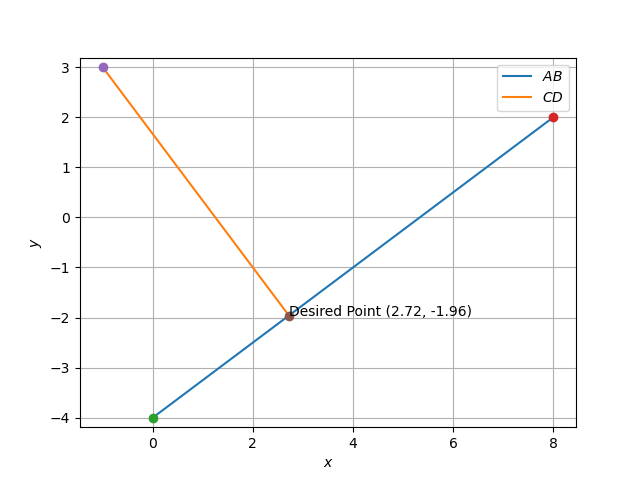
\includegraphics[width=\columnwidth]{./solutions/line_plane/42/Figure_1.png}
\caption{}
\label{fig:sol_line_plane_42}
\end{figure}

